\documentclass{article}%
\usepackage[T1]{fontenc}%
\usepackage[utf8]{inputenc}%
\usepackage{lmodern}%
\usepackage{textcomp}%
\usepackage{lastpage}%
\usepackage[head=40pt,margin=0.5in,bottom=0.6in]{geometry}%
\usepackage{graphicx}%
%
\title{\textbf{El regreso de Juan Guaidó en el marco de un nuevo ciclo y de la doctrina Monroe}}%
\author{LEOPOLDO PUCHI}%
\date{04/03/2019}%
%
\begin{document}%
\normalsize%
\maketitle%
\textbf{URL: }%
http://www.eluniversal.com/politica/34711/el{-}regreso{-}de{-}juan{-}guaido{-}en{-}el{-}marco{-}de{-}un{-}nuevo{-}ciclo{-}y{-}de{-}la{-}doctrina{-}monroe\newline%
%
\textbf{Periodico: }%
EU, %
ID: %
34711, %
Seccion: %
politica\newline%
%
\textbf{Palabras Claves: }%
NO\_TIENE\newline%
%
\textbf{Derecho: }%
2.1%
, Otros Derechos: %
\newline%
%
\textbf{\textit{Se entra en un nuevo ciclo, luego de haber fracasado el intento de cambio de gobierno que tuvo su momento culminante el sábado 23 de febrero}}%
\newline%
\newline%
%
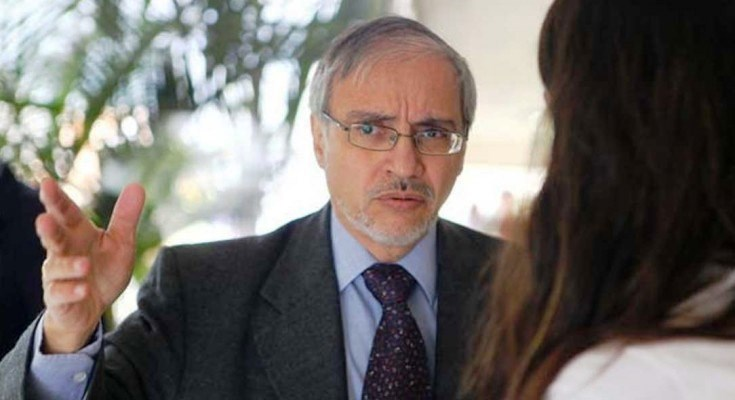
\includegraphics[width=300px]{EU_34711.jpg}%
\newline%
%
"Anuncio mi regreso a casa desde Ecuador”•%
\newline%
%
, declaró este domingo Juan Guaidó, luego de una gira por varios países.%
\newline%
%
•	El dirigente político afronta una posible orden detención cuando regrese a Venezuela por violar una prohibición de salida y por las acusaciones realizadas por la fiscalía con anterioridad.%
\newline%
%
•	Se desconoce si será arrestado o no, si será presentado al tribunal o si se realizará un juicio sin reclusión.%
\newline%
%
•	Desde la oposición han sido convocadas movilizaciones para lunes y martes, como forma de recibimiento y previendo que pueda ser detenido.%
\newline%
%
•	Se entra en un nuevo ciclo, luego de haber fracasado el intento de cambio de gobierno que tuvo su momento culminante el sábado 23 de febrero.%
\newline%
%
•	Elliot Abrams ha señalado que “no es posible fijar un día”, pero que no veía a Nicolás Maduro en el gobierno dentro de un año.%
\newline%
%
•	Mientras, John Bolton advirtió en una entrevista a CNN que continúan trabajando para crear “una coalición muy amplia para remplazar a Maduro”.%
\newline%
%
•	Bolton inscribió este propósito en el marco de la doctrina Monroe, que ha sido asumida por Donald Trump como eje de su política exterior hacia el continente en su disputa con Rusia y China. "Este es un país de nuestro hemisferio", dijo Bolton.%
\newline%
%
•	La doctrina Monroe expresada en el lema “América para los americanos” ha sido utilizada a lo largo del tiempo en función de los intereses estadounidenses en América Latina, incluso mediante intervenciones armadas.%
\newline%
%
•	Por esta razón, y para marcar una nueva política, en noviembre de 2013 el secretario de Estado de entonces, John Kerry, en la sede de la Organización de Estados Americanos afirmó: “La era de la doctrina Monroe ha terminado”.%
\newline%
%
•	En cuanto a las posibilidades de un diálogo o negociaciones, el asunto se continúa tratando en reuniones privadas, tanto de parte del Grupo de Contacto Internacional (GCI) como del Mecanismo de Montevideo. Para el 7 de marzo la comisión técnica del GCI dará su primer informe.%
\newline%
%
•	En el escenario público el diálogo poco ha avanzado. Jorge Rodríguez señalo que no estaban previstas elecciones presidenciales y dio a conocer varias propuestas que llevarían a una mesa de diálogo. Por su parte, la oposición insiste en un cambio de gobierno antes de cualquier proceso electoral.%
\newline%
%
\end{document}